\chapter{Misure di Valutazione}
Procediamo ora a descrivere i dataset contenenti dati di telemetrie registrati negli anni e resi pubblici in modo da poter sperimentare e migliorare gli algoritmi già presenti.

\section{Dataset ESA}

Il dataset di riferimento più importante per la rilevazione delle anomalie è quello fornito dall'ESA (European Space Agency) che conta dati di tre missioni. Di queste solo i dati di due vengono utilizzati per creare il benchmark, per le caratteristiche dell'insieme di dati; infatti in \textit{"Mission 3"} abbiamo: poche anomalie e per lo più banali, un gran numero di buchi di comunicazione e segmenti non validi.

Nell'articolo in questione i dati satellitari grezzi di \textit{"Mission 1"} e \textit{"Mission 2"} vengono preprocessati per renderli uniformi e quindi utilizzabili con la maggior parte degli algoritmi.

In questa fase utilizziamo OXI$^{\text{\cite{OXI_annotation_tool}}}$ per l'etichettatura collaborativa dei dati da cui si è potuto estrarre delle telemetrie che rappresentano periodi di funzionamento nominale e anomalo. Tutti i dati sono stati sottoposti ad una doppia fase di etichettatura e controllo.

I canali sono divisi tra "target" e "non target" dove quest'ultimi sono usati per gli algoritmi solo come informazioni addizionali. Un canale target, quello usato per rilevare le anomalie, è diviso in gruppi di dati con caratteristiche simili così da rendere più facile per l'algoritmo processarli ed interpretarli e, nel caso, allenarlo solo sul quel gruppo specifico.
\pagebreak

\begin{table}[h]
    \centering
    \begin{tabular}{|l|c|c|}
        \hline
         \textbf{}& \textbf{Mission 1} & \textbf{Mission 2}\\
         \hline
        \textbf{Channels} & 76 & 100\\
        Target/Non target & 58/18 & 47/53\\
        \hline
        \textbf{Telecommands} & 698 & 123\\
        \hline
        \textbf{Annotate Events} & 200 & 644 \\
        Anomalies& 118 & 31\\
        Rare Nominal Events &78  & 613\\
        Univariate/Multivariate& 32/164 & 9/635\\
        \hline
    \end{tabular}
    \caption{Configurazione Dataset ESA}
    \label{tab:costituzioneESA_dataset}
\end{table}

Possiamo osservare dalla Tabella \ref{tab:costituzioneESA_dataset} che la densità di anomalie in termini di punti di dati annotati, varia tra $0,57\%$ per la \textit{"Mission 2"} e $1,80\%$ per la \textit{"Mission 1"} questo va a confermare un'impronta più realistica rispetto ai dataset meno recenti che avevano una densità di anomalie estremamente più alta ed irrealistica.

\section{Motivazioni}
Il dataset ESA pecedentemente descritto porta alla risoluzione di vari problemi noti nell'ambito della rilevazione di anomalie.
Il primo problema come si evidenzia nei dataset \textit{NASA Soil Moisture Active Passive} (SMAP) e  \textit{Mars Science Laboratory} (MSL) i quali offrono brevi frammenti di segnali e comandi correlati da 55 e 27 parametri di telemetria, rispettivamente, con un totale di 105 anomalie annotate; infatti abbiamo una densità di anomalie irrealistica, alto numero di anomalie banali, verità di bse etichettate in maniera errate e una mancanza di corrlazione tra comandi e canali. Quindi è stato deciso che questi dataset non andrebbero usati per il benchamrking del rilevamento delle anomalie.
Il senondo problema invece rappresenta la mancanza di annotazione di eventi anomali, alcuni esempi sono gli insiemi di dati di \textit{Mars Express6} e \textit{NASA WebTCAD7}.

Il dataset ESA risolve i problemi elencati ma nasce come dataset di missioni su larga scala, le quali sono molto complesse e stabili portando con se problemi non più relativi alla distribuzione delle anomalie ma improntati verso problemi di esecuzione e potenza di calcolo.

Il dataset che intrudurremo dopo è concettualmente diverso, infatti affronta una missione ESA OPS\textunderscore SAT molto semplificata al fine di rendere più accessibile l'uso, oltre ad essere di dimensione considerevolmente minore.

Questo processo di apertura è reso anche tramite la sostituzione giornaliera dell'intero sistema software fino al sistema operativo del satellite così da consentire alle persone che sperimentano di caricare il proprio software a bordo e a terra. Per implementare questa funzionalità venne usato FDIR$^{\text{\cite{FDIR}}}$

Le telemetrie grezze sono caratterizzate da molte lacune nei dati ed altre imprecisioni, queste vengono curate da ingegneri ed esperti nei modelli di apprendimento automatico per rendere l'insieme di dati fruibile alla creazione di tecniche di rilevamento delle anomalie basate sui dati.
Una di queste modifiche è la seguente:

\begin{quote}
    Selezione e annotazione di verità di base (ground\textunderscore truth) di 2123 brevi frammenti di telemetria a canale singolo ossia serie temporali univariate$^{\text{\cite{10.1007/978-3-031-35995-8_21}}}$, registrate in 9 canali di telemetria.
\end{quote}

Infine questo dataset con il relativo benchmark e tutti i dati al suo interno disponibili è stato messo a disposizione per aiutare la comunità nella ricerca di nuovi approcci per la rilevazione delle anomalie, confrontandosi tra di loro in modo imparziale ed equo così da affrontare anche il problema della riproducibilità nell'ambiente dell'apprendimento automatico (dato che i dataset sono sono uniformati, l'ambiente di esecuzione diverso e varie metriche usate) 

Tutto ciò che è stato sviluppato con l'aiuto di questo dataset verrà convalidato con il lancio alla fine del 2025 del satellite successore OPS\textunderscore SAT VOLT (dopo averli distribuiti a bordo del satellite).


\section{OP-SAT Dataset}
Nel dataset OPS\textunderscore SAT sono contenuti i dati delle telemetrie del satellite OPS\textunderscore SAT dell'ESA (Figura \ref{fig:OP-SAT_satellite}). Questo satellite di tipo CubeSat aveva dimensione 3 unità (3U dove 1U=10cm$^3$), esso ormai non è più in orbita, era stato lanciato a Dicembre del 2019 con lo scopo di dimostrare l'elaborazione dei dati in orbita e di generare dati utili come immagini satellitari e telemetrie.

\begin{figure}[h]
    \centering
    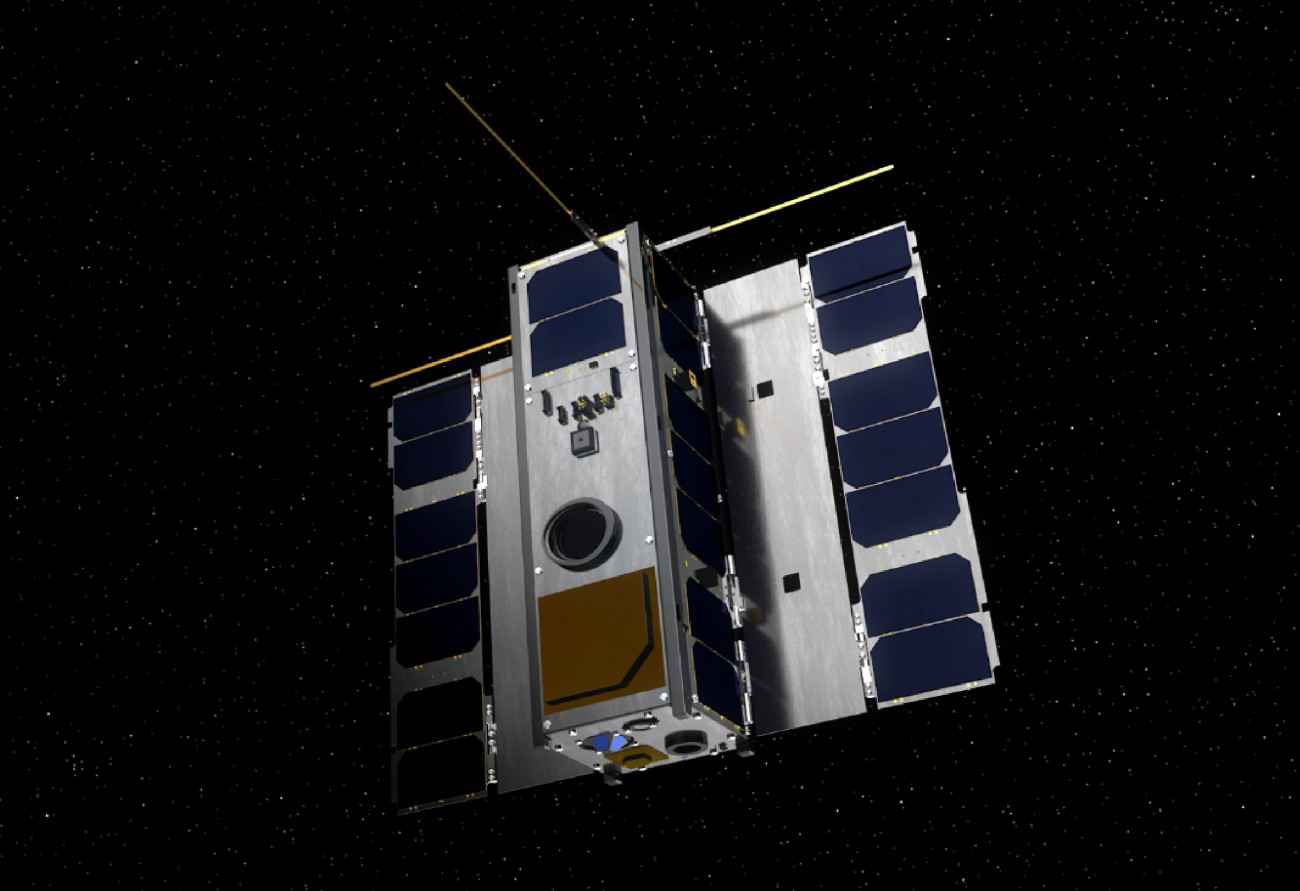
\includegraphics[width=0.5\linewidth]{images/Capitolo2/OP-SAT_satellite.png}
    \caption{Satellite OPS\textunderscore SAT. Fonte: European Space Agency}
    \label{fig:OP-SAT_satellite}
\end{figure}

Come nel dataset precedente anche qui i dati hanno bisogno di essere preprocessati per renderli fruibili alla maggior parte degli algoritmi (OXI$^{\text{\cite{OXI_annotation_tool}}}$). In questo caso sono state progettate 18 caratteristiche per l'attività di rilevamento delle anomalie, ossia sono stati estratti tratti significativi dai dati. Questo processo è chiamato Feature Extraction e serve per ridurre la complessità dei dati in ingresso rendendoli più significativi.

Tutti i segmenti ricavati rappresentano le sfide che dobbiamo affrontare con i dati delle telemetrie, ognuno di questi è composto da:
\begin{itemize}
    \item $\langle$\texttt{timestamp}$\rangle$: rappresenta il marcatore temporale nel momento della registrazione;
    \item $\langle$\texttt{channel}$\rangle$: è il nome del canale;
    \item $\langle$\texttt{value}$\rangle$: è il valore del segnale acquisito;
    \item $\langle$\texttt{label}$\rangle$: rappresentano le annotazioni certe, quelle annotate manualmente;
    \item $\langle$\texttt{segment}$\rangle$: rappresenta il numero consecutivo del segmento;
    \item $\langle$\texttt{sampling}$\rangle$: tasso di campionamento;
    \item $\langle$\texttt{train}$\rangle$: che indica se il segmento appartiene al training set.
    
\end{itemize}

Il dataset è stato diviso in una parte di allenamento, Training Set ($T$), ed una di test, Test Set ($\Psi$). Questi rappresentano rispettivamente i dati usati per l'allenamento del modello e i dati usati per fare le valutazioni delle performance dell'algoritmo.

\begin{table}[h]
    \centering
    \begin{tabular}{|l|c|c|c|}
        \hline
        \textbf{Classi} &\textbf{Training Set} ($T$) & \textbf{Test Set ($\Psi$)}&\textbf{Total} \\
        \hline
         Nominali& 1273&416 &1689 \\
         Anomalie& 321&529 &434\\
         \hline
    \end{tabular}
    \caption{Composizione Dataset OPS\textunderscore SAT}
    \label{tab:dataset_op-sat}
\end{table}

Le classi, nominali e anomalie, rappresentano rispettivamente segmenti che rispettano valori normali o attesi e segmenti invece che superano questi valori o discordano dai valori attesi.
Partendo dai benchmark effettuati su questi due dataset, analizzeremo le metriche e le prestazioni utilizzando in modo più specifico il secondo dataset (OPS\textunderscore SAT) che contiene dati più rilevanti per il nostro obbiettivo.

